% arara: pdflatex
% arara: biber if (missing("bbl") || changed("bib"))
% arara: pdflatex if (missing("bbl") || changed("bbl"))
% arara: pdflatex if (found("log", "Label(s) may have changed."))
\documentclass[portuguese]{beamer}
\usepackage[version=3]{mhchem}

\usepackage[utf8]{inputenc}
\usepackage[T1]{fontenc}
\usepackage{babel}
\usepackage{microtype}
\usepackage{xcolor}
\usepackage{anyfontsize}
\usepackage{pdflscape}
\usepackage{bbding}

% -- Tipo de letra
\usepackage{mathpazo}
%\usepackage{newpxtext}
%\usepackage{eulervm}
\usepackage{nimbusmono}

% -- Funções matemáticas extra
\usepackage{mathtools}
\usepackage{siunitx}

% -- Símbolos extra
\usepackage{amssymb}

\usepackage{textcomp}
\usepackage{gensymb}
\usepackage{cancel}

% -- Bibliografia
\usepackage[
	backend = biber,
	style = numeric,
	sorting = ynt
	]{biblatex}
\usepackage{fvextra}
\usepackage{csquotes}

% --  Definições de imagens
\usepackage{graphicx}
\graphicspath{{graphics/}}
\usepackage{caption}
\usepackage{subcaption}
\usepackage{afterpage}
\usepackage{tabularx}
%\usepackage[labelformat=empty]{caption}
\usepackage{multicol}
\usepackage{multirow}
\usepackage{booktabs}
\usepackage[export]{adjustbox}
\usepackage{caption}

% -- Desenhar circuitos elétricos e lógicos
\usepackage{tikz}
\usepackage{pgfplots}
\usetikzlibrary{arrows.meta,positioning}
\pgfplotsset{compat=1.5}
\pgfplotsset{table/search path = {data}}
\pgfplotsset{	/pgf/number format/use comma,}


\usepackage{todonotes}

%%%%%%%%%%%%%%%%%%%%%%%%%%%%%%
%Cenas do beamer

\addbibresource{../report/main.bib}
\addbibresource{main.bib}
\definecolor{istblue}{RGB}{0,157,224} % ist blue)

% símbolo de "certinho"
\def\checkmark{\tikz\fill[scale=0.4](0,.35) -- (.25,0) -- (1,.7) -- (.25,.15) -- cycle;} 
\mode<presentation>
{
  \usetheme{Madrid}       % or try default, Darmstadt, Warsaw, ...
  \usecolortheme{orchid} % or try albatross, beaver, crane, ...
  \usecolortheme[named=istblue]{structure}
  \usefonttheme{serif}    % or try default, structurebold, ...
  \setbeamertemplate{navigation symbols}{}
  \setbeamertemplate{caption}[numbered]
  \setbeamertemplate{itemize items}[circle] %ball,circle, square
  
} 

\setbeamertemplate{bibliography item}{\insertbiblabel}
\setbeamertemplate{caption}{\raggedright\insertcaption\par}

\setbeamertemplate{caption}[numbered]
\setbeamerfont{institute}{size=\Large}
\setbeamerfont{date}{size=\small}
\setbeamerfont{author}{size=\small}




\title[Radar MIMO]{Radar MIMO}


\author[MEAer -- Sistemas de Radar]{
  João Gonçalves \texttt{81040} \and Daniel de Schiffart \texttt{81479} 
    }

\institute{Sistemas de Radar}
\date{Dezembro de 2018}
\setbeamertemplate{footline}
{
  \leavevmode%
  \hbox{%
  \begin{beamercolorbox}[wd=.333333\paperwidth,ht=2.25ex,dp=1ex,center]{author in head/foot}%
    \usebeamerfont{author in head/foot}\insertshortauthor
  \end{beamercolorbox}%
  \begin{beamercolorbox}[wd=.333333\paperwidth,ht=2.25ex,dp=1ex,center]{title in head/foot}%
    \usebeamerfont{title in head/foot}\insertshorttitle
  \end{beamercolorbox}%
  \begin{beamercolorbox}[wd=.333333\paperwidth,ht=2.25ex,dp=1ex,right]{date in head/foot}%
    \usebeamerfont{date in head/foot}Trabalho de síntese\hspace*{2em}
    \insertframenumber{} / \inserttotalframenumber\hspace*{2ex} 
  \end{beamercolorbox}}%
  \vskip0pt%
}

%%%%%%%%%%%%%%%%%%%%%%%%%%%%%%%%%%%%%%%%%%%%%%%%%%%%%%%%%%%%%%
\begin{document}

\begin{frame}
    \begin{figure}
	
\includegraphics[width=0.5\linewidth]{graphics/tecnico_logo.png}
    \end{figure}
    \titlepage
\end{frame}
\setbeamertemplate{section in toc}[circle]
\begin{frame}{Conteúdo}
  \tableofcontents
\end{frame}

\section{Introdução}

\section{Conceito MIMO}

\begin{frame}{Conceito MIMO}
  \begin{figure}[]
	\centering
	\begin{minipage}[t]{0.5\linewidth}
	  \centering
	  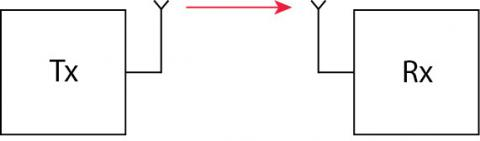
\includegraphics[width=0.7\linewidth]{com1.jpg}
    \end{minipage}%
    \begin{minipage}[t]{0.5\linewidth}	
	  \centering
	  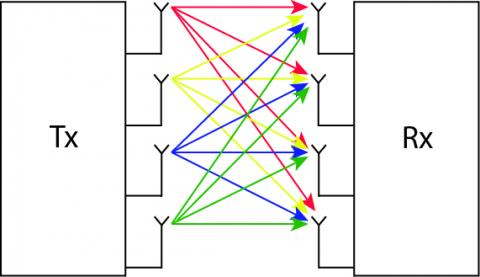
\includegraphics[width=0.7\linewidth]{com2.jpg}
    \end{minipage}%
	\caption{Sistema SISO e MIMO. Fonte: \cite{swantennas}.}
	\label{fig:antenas}
  \end{figure}
\end{frame}

\begin{frame}{Radar MIMO}
  \par
  {\large Radar MIMO -- \textit{multi-input multi-output}} 
  \begin{itemize}
	\item Generalização do radar multiestático.
  \end{itemize}
  \begin{figure}[]
	\centering
	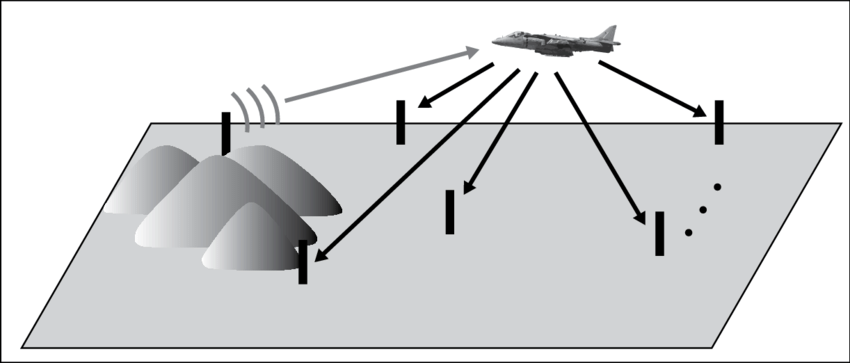
\includegraphics[width=0.8\linewidth]{../report/graphics/multistatic.png}
	\caption{Radar multiestático. Fonte: \cite{mimoradarbook}}
	\label{fig:mono}
  \end{figure}
\end{frame}

\section{Radar MIMO}

\begin{frame}{Radar MIMO}
  \begin{itemize}
	\item Radar MIMO coerente -- generalização do mono-estático.
  \end{itemize}
  \begin{figure}[]
	\centering
	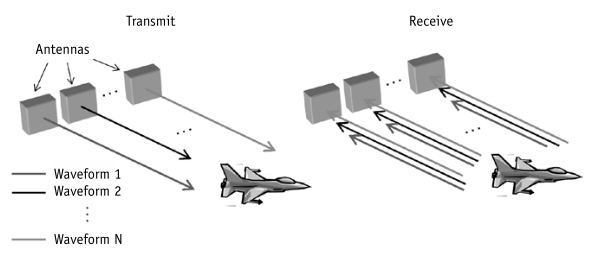
\includegraphics[width=0.7\linewidth]{../report/graphics/concept.png}
	\caption{Radar MIMO coerente. Fonte: \cite{mimoradarbook}.}
	\label{fig:concept}
  \end{figure}
\end{frame}



\section{Processamento de Sinais}

\section{Aplicações}

\section{Perspetiva Histórica}

\begin{frame}{Referências}
  \printbibliography
\end{frame}

\end{document}

